
\documentclass[11pt]{article} 
\usepackage{styles/preamble_diss}

\title{PhD materials}
\author{Kirill Borisov}

\begin{document}

\begin{titlepage}
\maketitle
\end{titlepage}

\tableofcontents
\newpage

%\section{Abstract}
%\section{Introduction}
\subsection{What are spectra and why we need them}

According to quantum theory in physics, all quantum systems have a finite or infinite number of quantum states, distinct by energy level. Energy levels are usually eigenvalues of an energy operator, most commonly - the full energy operator, or Hamiltonian, which is the sum of potential and kinetic energy operators.

Quantum systems can undergo transitions between quantum states with different energy, but the energy conservation law obligates quantum system to use some energy carrier to fill the energy gap between the different quantum states. One of the most abundant energy carriers in the universe is the photon, a particle which gives rise to the macroscopic phenomena of electromagnetic radiation and electromagnetic force.

Atoms, poly-atomic molecules and ions in space or in some laboratory experiments can be treated as isolated quantum systems. They undergo quantum transitions, absorb and emit photons. Photons, or electromagnetic waves, can travel large distances until they hit our detectors, where their energy is measured. A set of measured transitions plotted as intensity versus energy is called a spectrum. 

Spectra are objects of study in spectroscopy. We analyze experimental spectra to learn transitions parameters of molecules in known laboratory conditions. This is what laboratory spectroscopists are doing. We also analyze experimental spectra to find characteristic transitions of particles with known transition parameters, i.e. identify particles by their "fingerprints". This is what astrophysicists are doing. 

The latter particles often exist in in unknown conditions, e.g. unknown temperature and gas pressure in space. Then there is an additional task to find out these conditions, to learn things about space by just examining spectra of molecules, atoms and ions. We can learn about the constituents of stars, planets and giant clouds of gas and dust in space, about their motion, heating and cooling processes and chemical reactions. We can learn things about the birth and death of stars and galaxies.

\subsection{Basics of molecular spectroscopy}

In this work, I concentrate on spectra of molecules.

\subsubsection{Born-Oppenheimer approximation}

In the Born-Oppenheimer approximation the full energy $H$ of a molecule can be written as a sum of:
\begin{enumerate}
	\item potential energy of the electrons in the potential well of much slower nuclei ($H_e$)
	\item kinetic energy of the electrons, which is negligible because of comparably very low mass of the electrons
	\item kinetic energy of the nuclear skeleton:
	\begin{enumerate}
		\item translational, which can be set to zero for a single molecule without loss of generality
		\item vibrational ($H_v$)
		\item rotational ($H_r$)
	\end{enumerate}	
\end{enumerate}

All these operators (except the one for translational energy) have discreet spectra. The orders of magnitude in energy eigenvalue differences are the following for each operator:
\begin{itemize}
	\item $H_r$: microwave and sub-millimeter (terahertz, far-infrared) regions, approx. 300-3'000'000 $MHz$
	\item $H_v$: near- and mid-infrared regions, approx. 1'000-10'000 $cm^{-1}$
	\item $H_e$: visible region and higher energies
\end{itemize}	

Electronic spectra were the first to be thoroughly studied, initially spectra of single atoms in visible light, ultraviolet and x-ray. There were some experiments with photo plates and alkali metals. Modern electron spectroscopy uses bremsstrahlung and other sources of UV and x-rays.

According to the classical interpretation of molecular vibrations, each chemical bond in a molecule vibrates at a frequency characteristic of that bond. A group of atoms in a molecule (e.g., $CH_2$) may have multiple modes of oscillation caused by the stretching and bending motions of the group as a whole. 

Vibrational frequencies for most molecules correspond to the frequencies or energies of infrared light. Infrared lasers and infrared telescopes are used to study organic compounds in laboratories and in space. Information about the sample composition in terms of chemical groups present and information about bond lengths can be obtained in these experiments. 

Microwave spectroscopy deals with low-energy quantum transitions. Firstly, this helps to study cold regions of space, because in regions with low ambient energy only low-energy quantum states are being excited - rotational states. Secondly, all detectors and experiments, while consistently getting better, are limited by their relative resolution, which is the ratio between energy (frequency) resolution and the actual energy of recorded spectra. This implies that spectra with lower energy can reach better resolution then their electronic and (ro-)vibrational counterparts. Also, pure rotational transitions are well suited to study cold interstellar objects, in which mostly only rotational levels of molecules are populated. 

Modern microwave spectroscopy uses tunable power sources with small frequency bandwidth, big signal to noise ratio, high stability etc., which are called synthesizers or local oscillators.

The THz frequency band is located between the spectral regions of microwave and infrared wavelength. It is one of the most unexplored regions in the electromagnetic spectrum, because powerful, tunable, monochromatic radiation sources have been practically not available. Enormous technical progresses in the development of such light sources over the last years give astronomers and spectroscopists increasingly access to this frequency region. 


\subsubsection{Complexity of a molecule and its spectrum}

In this work, I concentrate on microwave (rotational) spectroscopy of molecules with approx. 2-10 nuclei. 

Rotational spectra with more nuclei become increasingly more complex. Firstly, most \lq\lq{}big\rq\rq{} molecules are asymmetric tops. Secondly,  molecules that have many atoms with many degrees of freedom posses lots of possible vibrational excited states and possibly many isomers and conformers. They have many Hamiltonian parameters, distortions and irregularities. Some of them are "floppy" and don't have an adequate quantum model at all.

Complex spectra have great line density and many blended lines.

\subsubsection{Human effort}

In this work, by saying "human effort" I primarily mean time - working hours of scientific stuff spent on conducting experiments and on the analysis of each species in each experiment. During analysis, people usually have to look through raw spectroscopic data several times, as well as they have to interact with spectroscopic software with the computer mouse, press many buttons etc. All of this consumes a lot of time a requires concentration, because mistakes are often crucial for the end result and also they can be hard to track. There are several general ways to reduce human effort:
\begin{itemize}
 	\item reduce the amount of "clicks" or other actions with the mouse and keyboard
	\item delegate some work to automatic computer algorithms 
	\item make software tools and their graphical user interfaces more user-friendly
	\item introduce better guidelines for people to make less mistakes
	\item mistakes should be less critical, i.e. easier to locate and undo
\end{itemize}



\section{The way towards automated molecular spectra analysis}

In this chapter the \lq\lq{}standard fitting procedure\rq\rq{} of rotational molecular spectra analysis is described, with details of that procedure, existing tools and methods. That leads to a discussion of new approaches with a focus on automation (reducing human effort). Examples are given with spectra of three molecules with increasing complexity of their spectra: OCS, vinyl cyanide (acrylonitrilie) and thiazole. Among them OCS is the simplest case, a linear top; the other two molecules are asymmetric tops: vinyl cyanide has a slightly crinkled carbon chain with a cyano (CN) group at the end and hence it is a nearly prolate top; thiazole is a ring molecule, oblate but highly asymmetric ($\kappa=-0,166$).   

\subsection{Molecular models and a standard fitting procedure}

In laboratories, we usually conduct experiments under known physical conditions $\mathfrak{C}$ (temperature, pressure, radiation etc.) until a phenomenon is understood good enough. This understanding is described in a \emph{model} of the phenomenon. In particular, laboratory molecular spectroscopy involves building a model of the molecule or molecular ion (below we use the word \lq\lq{}molecule\rq\rq{} for both cases), which can be later used to predict how observations of those molecules look like under various conditions of observations and depending on conditions of observation. Thus, observational data under unknown conditions $\mathfrak{C}'$ can be compared with theoretical predictions and $\mathfrak{C}'$ can be deduced. Again, the model of the molecule is the knowledge we obtain from our laboratory experiments. 

The simplest way to obtain this knowledge would be to memorize experimental results for every possible set of conditions $\mathfrak{C}$. Of course, it is unpractical. Therefore we usually need to summarize experimental data in relatively simple model, fully defined by only a few adjustable parameters $p_1, ..., p_n$. There is an obvious trade-off between prediction quality and model complexity.

A model of a molecule is a mathematical object $M(\cdot | p_1, ..., p_n): \mathfrak{C} \rightarrow \Pi$, where $\mathfrak{C}$ are all possible physical conditions of observation, $\Pi$ are possible predicted spectra and $p_1, ..., p_n$ are internal model parameters. The model $M$ is constructed by \emph{fitting} its parameters to experimental data, i.e. optimizing  $p_1, ..., p_n$ in a way that predicted transitions are in some sense close to observed lines.  

Data can origin from different kinds of experiments. While all experiments in the field of molecular spectroscopy involve detectors of electromagnetic radiation, other conditions vary: there may be a heating or cooling system for temperature control, there may be an electric field for Stark measurements etc. Approaches to spectral analysis vary accordingly. 

There is, however, a commonly used fitting procedure, that we exclusively treat in this work. We call the it the \lq\lq{}standard fitting procedure\rq\rq{} (SFP). This is its  general outline:

\begin{enumerate}
	\item Initialization: an initial model $M_0$ -- an initial set of parameters  ${p_1}, ..., {p_{n(0)}}$ is made by guessing, extrapolation existing models or by \lq\lq{}ab inito\rq\rq{} quantum calculation software (0). Here $n(0)$ is the initial amount of parameters; $n$ can change later. 
	\item Fitness function construction. The fitness function will optimize model parameters in a later step by its value $\phi(M)$.
	\item Fit parameters selection. There is a decision to be made about which parameters to actually fit, which to keep constant and which parameters to add or even remove from $M$ at each iteration.
	\item Improvement of parameters ${p_1}_i, ..., {p_{n(i)}}_i \rightarrow {p_1}_{i + 1}, ..., {p_{n(i)}}_{i + 1}$ by means of local or global optimization of $\phi(M)$. Here $i$ is the iteration index.
	\item Repeat (2) through (4) until some stop condition is reached.
%Following tools are used here:
%	\begin{itemize}
%		\item The de facto standard tool for rotational and (ro-)vibrational spectroscopy are Pickett's SPFIT and SPCAT (0). They input and output simple text files in Pickett format. The CDMS catalog entries are basically output Pickett files. Many third-party software tools use Pickett as their core.
%		\item Colin Western's PGOPHER is often used, being an all-in-one program for the whole SFP with additional features (0).
%		\item Models with some complications require other fitting software, e.g. to take internal rotation into account (0). 
%	\end{itemize}
	
\end{enumerate}

We see that the SFP may or may not be iterative. A non-iterative approach (a single iteration) is used if all experimental data can be fitted at once \emph{and} in an unambiguous way. When one of those two requirements are broken, an iterative approach is used. 

An iterative SFP is similar to the expectation-maximization algorithm in statistics. The latter is also iterative and is used when a model is dependent on unobserved latent variables. In our case, possible ambiguity in the way how experimental data must be treated can be expressed in terms of an unobserved variable on which a special function depends, which we call metric.

Let $a \in \mathfrak{A}$ be the unobserved variable. Then there is not only the model $M$ that determines the fit, but a pair $(M, a)$, and both must be optimized. A metric on $\mathfrak{A}$, $f(\cdot | M): \mathfrak{A}~\rightarrow~\R$ (or more generally, $f(\cdot | M): \mathfrak{A}~\rightarrow~Q$ with an arbitrary ordered quality space $Q$), would assess the quality of both the model with its parameters and $a$. %The latter represents treatment of experimental data and can vary from iteration to iteration.
The function $\phi$ from step (2) can be constructed in the sense of binding $a$: $\phi(M) = f(a | M)$.

Approaches to the SFP can be now classified by nature of $\mathfrak{A}$.
\begin{itemize}
	\item Global fits. All experimental data is used at once in a (global) parameter optimization. No hidden variables.
	\item Fits with spectral line assignment (two-quantum-state fits). $\mathfrak{A}$ are candidate spectral line assignments.
	\item Fits with quantum state assignment (one-quantum-state fits). They use spectral lines to reconstruct individual quantum states from combination differences. $\mathfrak{A}$ are individual quantum state assignments.
\end{itemize}

Let's consider fits with spectral line assignment. Spectral line assignment is by now a poorly automated and challenging task; nevertheless, fits with spectral line assignment are the most commonly used type. In a database like CDMS or JPL you find entries on molecular models with ready assignments.

\subsection{Spectral line assignment}

%A spectrum line is an image of a quantum transition between two quantum states (see Introduction). 

Imagine two sets of spectral lines: experimental lines $E$ and predicted lines $P$ (the latter are predicted by the model at some point in time). They are also often call observed lines and calculated lines (\lq\lq{}obs and calc\rq\rq{}). Each  line in $E$ is defined as a tuple $(x_e, ...)$ of peak position (frequency) and its other properties, such as intensity or width. Here, the peak position $x_e$ is unique. Often $E$ is extracted from raw experimental data with a peak finder. Each line in $P$ is also defined as a tuple $(q, x_p, ...)$ of predicted transition frequency $x_p$, identifier $q$ and other properties of the transition. The identifier $q$ must be unique among $P$. Commonly, transition quantum numbers serve that purpose. Frequencies $x_p$ may be not unique due to degeneracy. 

We call an \emph{assignment} (denoted $a$) a surjection from $P_a \subset P$ to $E_a \subset E$, which is a mapping $g_a(\cdot): P_a \rightarrow E_a$ or, equivalently, a set of tuples: 
\begin{equation}
\label{def_assignment}
	a \defeq \{(q, x_e, ...): (q, ...) \in P_a; (x_e, ...) = g_a((q, ...)) \in E_a\}.
\end{equation}

In nature, lines $E$ and $P$ are the same thing - transitions of a molecule. There is a real transition frequency $x$, so that both $x_e$ and $x_p$ are estimates $\hat x$. The discrepancy between  $x_e$ and $x_0$ arises from the imperfectness of experiments; the discrepancy between $x_e$ and $x_p$ (or between $E$ and $P$) arises from the imperfectness of experiments \emph{and} $M$. We imply that there is one, and only one, correct and complete assignment $a_0(E, P)$ for any given $E$ and $P$, among the possible assignments $\mathfrak{A}$. 

A metric $f(\cdot | M): \mathfrak{A}~\rightarrow~Q$ with some quality space $Q$ can be used to assess the quality of an assignment $a$ for the model $M$. %As said before, in practice $f$ will almost inevitably assess both $a$ and the underlying model.

In case $a = a_0$, function $f$ can be indeed used to optimize the model parameters $p_1, ..., p_n$. It should be using some distance between $E$ and $P$. If only transition frequency is taken into account, the RMS of the \emph{residuals} is commonly used:
\begin{equation}
\label{def_rms}
	f_{RMS}(a) \propto \sum (x_e - x_p)^2\;{\rm with}\;a\;{\rm from}\;\ref{def_assignment}
\end{equation}
Due to the commonly normal distribution of $x_e$, residuals $x_e - x_p$ (often called \lq\lq{}obs minus calc\rq\rq{}) can be seen as estimates of $x_p - x_0$. The least squares fitting method depends on this to give reasonable $M$. 

Alas, there is no way to be certain about if $a = a_0$, because $a$ is not directly observable. I will therefore often write about \lq\lq{}almost correct\rq\rq{} assignments, meaning those that share almost all $(q, x_e)$ pairs with $a_0$ except for only a relatively small amount of those pairs. %Additionally, experimental spectra often contain mixtures of $m > 1$ different species. In that case, there may be several correct assignments ${a_0}_i$, $i = 1, ... m$.
A line assignment improvement step in fitting means adding pairs $(q, x_e)$ to $a$ that look good, or removing them if some of them seem to be wrong. But this has do be done differently depending on the spectrum itself and depending on $|a|$, i.e. how many lines are already assigned. 

 % a peak finder will find $E$ as a mixture of different $E_1, ... E_m$. Some peaks can also be blended between species, i.e. possibly $\exists e \in E: e \in E_i, e \in E_j, i \neq j$. Probably, separate models $M_1, ..., M_m$ and, accordingly, separate $P_1, ..., P_m$ will be available. But each of $P_1, ..., P_m$ (or at least the first one) has to be assigned to the whole experimental data $E$. There is still one (and only) correct and complete assignment ${a_0}_i$ for each $P_i$, $i = 1, ..., m$. But starting from some model ${M}_i$ we might under some circumstances get a partly correct assignment for another model, i.e. $a \approx {a_0}_j$, $j \neq i$.

%A pair $(M, a)$ represents the current analysis status rather then $M$ alone. 

Depending on $|a|$, we distinguish \emph{stages} of spectral line assignment: early stage, intermediate stage and late stage.

The early stage of assignment usually means assigning at least first $n_0$ lines -- as much as the initial number of model parameters -- and ideally several times that amount. This may be challenging, because initial parameters may yield $P$ very different from $E$ and spectral lines may even not be in the correct order, so that assigning to the nearest in sense of $|x_p - x_e|$ often results in totally wrong assignments, which may be noticed only later and rise a need to go many steps back. 

The late stage of assignment is the easiest one. Experimental and simulated lines already match so well that simply assigning to the nearest in sense of $|x_p - x_e|$ gives a correct result and continuously improves $M$ with $|a|$ going up. Large frequency regions can be assigned at once. The only thing to worry about is the possible need to add more parameters to the model, e.g. Hamiltonian distortions to describe transitions with higher frequencies and quantum numbers.  

The intermediate stage is everything in between. You may try assigning simulated lines to nearest experimental peaks, but you still have to select one from several possible options sometimes, and eventually traverse a decision tree to get the best assignment.

For assignment of rotational spectra to models where transitions are labeled with quantum numbers $q = (J', ...; J'', ...)$, lines are commonly assigned in groups or series of two different kind:
\begin{itemize}
	\item Groups of transitions with the same value of quantum number $J'$ or $J''$ ($K$-ladders). 
% TODO: (in symmetric and asymmetric tops often called $K$-ladders because of splitting by different $K_a$ and/or $K_c$ values). -> move to introduction
The overall direction of traverse is from lower frequencies to higher frequencies, which correspond with going from lower $J$ values to higher $J$ values.  
	\item Groups of transitions with the same $K_a$ or $K_c$ value, which resemble linear top spectra as part of more complex spectra.
\end{itemize}

Spectral line assignment requires sharp eyes: visual tools are used, such as SMAP, ASCP, PGOHPER. Since it is poorly automated, an obvious idea would be to start reducing human effort from here.

\subsection{AUTOFIT}

AUTOFIT is a technology of automated spectral line assignment and a software with the same name originally developed by the Pate group. 

The original AUTOFIT is written in Python as a wrapper for Pickett SPFIT and SPCAT programs. It is primarily designed for the early stage of assignment and restricts to models of rigid asymmetric tops with 3 rotational constants (A, B, C).  No additional constants are added during the process (except for so-called refinement in the very end, which is actually not automatic). These can be considered as major drawbacks that are lifted in the fairly new AUTOFIT feature inside PGOPHER. 

The PGOPHER version allows to fit all models that can be built in PGOPHER, i.e. linear, symmetric and asymmetric rotors with pure rotational constants  or ro-vibrational constants, including distortions.

\subsubsection{Working principle of AUTOFIT}

With some user input, AUTOFIT constructs a set of candidate assignments $\mathfrak{A}$. For each assignment $a \in \mathfrak{A}$ the software evaluates a metric $f(\cdot | M):~\mathfrak{A}~\rightarrow~Q$, where $Q$ is some ordered quality space. The output is a list of assignments sorted by $f(a) \in Q$, where the upper rows are, under certain conditions, more likely to be better assignments or even (almost) correct assignments than the lower rows. Of course, the magic hides in ways to define $\mathfrak{A}$ and $f$. These are the classical steps of AUTOFIT:

\begin{enumerate}
	\item A peak finder is run on the experimental spectrum to construct $E$. Original AUTOFIT provides a built-in simple peak finder, which find all local maxima above a certain threshold on the Y axis, independent on the peak width or anything else. 
	\item Provided an initial model $M_0$, an initial $P_0$ is generated (e.g. with SPCAT). Already assigned lines may be present before auto fitting -- the current assignment $a_{cur}$.
	\item So-called fit transitions $S \subset P_0$ are selected by the user - typically as much as the number $n$ of model parameters. Also a search window size $\Delta s$ in frequency units is selected by the user.
	\item So-called check transitions $C \subset P_0$ are selected by the user. Also a check window size $\Delta c$ in frequency units. 
		\item Each transition $(q, x_p, ...) \in S$ is assigned to an experimental line $(x_e, ...) \in E$ if $|x_p - x_e| < \Delta s$. All combinations are tested; the set of all such sub-assignments is called $\mathfrak{a_s}$. For example, if there are 30 experimental peaks inside $\Delta f$ around each of the search transitions, $|\mathfrak{a_s}| = 30^{n}$ for fitting $n$ model parameters. If $\mathfrak{a_s}(S, E, \Delta s) = \emptyset$, AUTOFIT is considered to have failed. 
		\item $\forall a_s \in \mathfrak{a_s}$, $a_{cur} + a_s$ are used in trial fits of the model $M$ (e.g. with SPFIT). This gives candidate models $M(a_s)$ and altered predicted transition sets $P(a_s)$. Based on labels (quantum numbers) of the predicted transitions, the initial fit transitions $S \in P_0$ and check transitions $C \in P_0$ are mapped into altered versions $S' \in P(a_s)$ and $C' \in P(a_s)$. 

The AUTOFIT version in PGOPHER also provides an option to restrict parameters $p_1, ..., p_n$ of $M$ inside an n-dimensional cube. If for any ${a_s}_0$ parameters of $M({a_s}_0)$ evade from this cube, this sub-assignment is discarded.  It can speed up things drastically because of pruning at early fitting iterations.    
		\item Transitions $(q, x_p, ...) \in C'$ are assigned to \emph{nearest} experimental lines $(x_e, ...) \in E$ if $|x_p - x_e| < \Delta c$. This sub-assignment is unique and based on $a_s$, so we call it $a_c(a_s)$. Zero or more check transitions are assigned, let's call this quantity $n_{OK}$.
		\item  The candidate assignments set $\mathfrak{A}$ is constructed as $\{a_{cur} + a_s + a_c(a_s)\}\,\forall a_s \in \mathfrak{a_s}$.
	\item Assignment metric $f(\cdot | M):~\mathfrak{A}~\rightarrow~Q$ is defined as a pair $(f_1, f_2)$, where $f_1 = n_{OK}$ is the amount of assigned check transitions, and $f_2 = f_{RMS}(a_c)$ is the RMS of assigned check transitions' deviations, $f_{RMS}$ defined in \ref{def_rms}. 
	\item AUTOFIT output contains pairs $(f_1, f_2)$; it is ordered first descending by value of $f_1$ and then ascending by value of $f_2$. The implied idea is that better assignments have more check transitions assigned, even with larger RMS values. 
\end{enumerate}

As you can notice, the check transitions are \emph{not} being fit at all in the classical algorithm. This saves computation time at the cost of getting \lq\lq{}incorrect\rq\rq{} obs minus calc values for the full candidate assignment in the sense of not being obtained from a best fit, which one could expect.

%There are still some degrees of freedom left in this algorithm: how do we select these meta parameters for AUTOFIT: $S$, $C$, $\Delta s$, $\Delta c$? Here are some considerations.

\subsubsection{Selecting meta parameters of AUTOFIT}

\paragraph{Search windows size.}

If there is an error estimate $\widehat {\Delta \beta} = (\widehat {\Delta p_1}, ..., \widehat {\Delta p_n})$ in the model parameters which are currently fit, one may calculate an according deviation estimate $\widehat {\Delta s}_i$ in the frequency position of fit transitions  $s_i \in S$ and take $\Delta s = \max \widehat {\Delta s}_i$. % This approach is called a \emph{mutation test} in this work. 
A maximum over all search transitions is taken because only a single search window size is to be selected in PGOPHER. Actually, it is more time efficient to define individual search window sizes $\Delta s_i$ for each search transition.

% The $\widehat {\Delta \beta}$ could be obtained from a previous least squares fit, but it could only be interpreted as a statistical error if the assignment didn't change since then, which doesn't hold -- AUTOFIT adds candidate assignments to the previous one.

In practice, $\widehat {\Delta \beta}$ can be experience values for ab initio calculated values, as classical AUTOFIT is normally used as a fist step at the early stage of the assignment. After the first lines have been assigned, $\widehat {\Delta \beta}$ should be drastically reduces, but I cannot think of a simple analytical way to do this.

If the fit transitions sit in the search window and they are observable, $S$ will be assigned correctly with certainty. But there can be practical situations when some $s \in S$ are not observable in given experimental data even if expected to be.

\paragraph{Fit transitions set.}

With same $\Delta B$, we will usually get smaller $\Delta s$ for fit transitions with lower frequencies (lower quantum numbers). The best in this sense are transitions between low-lying energy levels, which are well populated in supersonic jet experiments, but not at room temperature. AUTOFIT was originally designed for low temperature experiments, and if we want to analyze data from room temperature experiments, we get a trade-off between $\Delta s$ and peak intensities (signal-to-noise ratio). Experience shows that with modern spectrometers at room temperature, the region around 100 GHz is a good starting point. 

The entire set $S$ of fit transition must contain information on the entire set of currently fitted parameters for the optimization problem to be well defined.

\paragraph{Check transitions set.}

This may be the easiest meta  parameter to choose. There must be enough check transitions to reject wrong assignments, any additional assigned check transition reduces the probability of incorrect assignment; search time has only a linear dependent on their amount, so more is just better than less. The whole group of lines that is to be assigned, expect for $S$, can be made $C$.

\paragraph{Check window size.}

The AUTOFIT manual suggest to choose it equal to the experimental peak width. But a careful look reveals that a $\Delta c$ value equal to the experimental peak width is only the minimum value for $\Delta c$. This approach only covers obs minus calc  with zero mean, $\mean (x_e - x_p) = 0$, where $x_e$ considered stochastic variables. Taking the real transition frequency $x_0$ again, $\mean (x_e - x_0) = 0$ usually holds (and also $x_e$ have a normal distribution). But that doesn't cover \lq\lq{}systematic\rq\rq{} deviations with nonzero mean, which may be introduced to $x_p$ by a non-adequate model.

Commonly  model parameters are coefficients of a Hamiltonian eigenvalue expression. It contains some main terms and some terms derived from a perturbation Hamiltonian. These perturbation terms form an endless series, which has to be truncated adequately at some point. In particular, PGOPHER works with rotor Hamiltonians. If, for example, the rotor is a linear molecule, the predicted line frequencies will be expressed as:
\begin{multline}
\label{linear_eigenvalues}
x_p(J', J''\, |\, v_0, A', A'', D', D'', ...) = \\
= v_0 + B'J'(J'+1) - B''J''(J''+1) - D'{J'}^2(J'+1)^2 + D''{J''}^2(J''+1)^2 + ... 
\end{multline}

There are two possible deviation sources in connection with this, arising from both insufficient and over-sufficient amount of experimental data in the fit:
\begin{enumerate}
	\item Expression \ref{linear_eigenvalues} may be truncated at a too early term, so that the model doesn't describe experimental data at high values of $J$ adequately;
	\item Expression \ref{linear_eigenvalues} has enough terms to describe the data; however, there is not sufficient data for the higher order terms to be well defined. 
\end{enumerate}

%What systematic error arises from truncating this expression up to $D$ with large-$J$ experimental data in the fit? 
For the least squares method, an exact formula can be obtained for a systematic error $\delta$ between the current and the next order precise models. This formula will depend on the (candidate) assignment $a$. The classical AUTOFIT defines $\Delta c$ before test-assigning the fit transitions, but one could modify the sequence and (automatically) select $\Delta c$ for each candidate assignment of fit transitions.  

% The same is the case for insufficient data and poorly defined $D$: a formula can be obtained in the least squares method case for the deviations, but they will depend on the $D$'s uncertainty, which in turn depends on the assignment $a$. There deviations usually cannot be neglected in classical AUTOFIT because, as mentioned However, in classic AUTOFIT only a model $(M, a_s)$ is being fit. Best fit residuals for the model $(M, a)$ appear only after an additional fitting cycle. Thus the RMS values in AUTOFIT output are generally too high values.

% From this minimum value it can be increased until some stop condition is reached, e.g. until a test assignment doesn't change anymore or until there is a distinct correct assignment in the AUTOFIT output. 
%Also $\Delta s$ can be increased in a similar fashion, starting from an initial guess. 

Next, I wanted to analyze the output of AUTOFIT and develop a method to distinguish correct and \lq\lq{}almost correct\rq\rq{} assignments. For this task, I did some tests with different molecules in PGOPHER. 

\subsubsection{Workflow in PGOPHER}

PGOPHER is comprehensive software with many features. It facilitates fitting and spectrum line assignment for rotational and ro-vibrational spectra on every stage of assignment. Details of workflow in PGOPHER are described in its online manual. To sum up what we need in this work, here is how standard fitting goes in PGOPHER: 
\begin{enumerate}
	\item Current assignments are usually kept in the Line List window. New transitions have to first be added there, either by clicking them in the main windows or by adding certain groups from the Transitions window (the latter is more effective). 
	\item Then they have to be assigned in some way to $E$ peaks of the Overlays: manually, with the Nearest Lines Plot or the AUTOFIT option.
	\item The Fit button in the the Line List windows performs one cycle of least squares fitting of rotor parameters specified in the Constants window.
	\item The Residuals window will appear, where one can assess the quality of the model-with-assignment $(M, a)$.
\end{enumerate}

% For the late stage of assignment the Transitions window and the Line List window both have got a Nearest button, one click on which will assign selected transitions to nearest experimental peaks. The Accept input box in the Line List window serves here as a threshold or maximal frequency deviation. 

Since 2017 the early stage of assignment is reinforced by AUTOFIT. You can right click on transitions from the Line List window and select options Mark for Autofit and Mark as Check. These will be the fit and the check transitions respectively. The Accept input box in the Line List window serves here as $\Delta c$ and the Window input box in a special Autofit window serves as $\Delta s$. Rotor parameters or constants can be confined inside a hypercube -- use the StdDev column in the Constants window.

The output assignments will be listed in the Autofit window as rows in a table. Each row is a separate assignment. On click on an output row the selected assignment is applied. Values of the fitness function $f = (n_{OK}, {RMS})$ are given in the first two columns: nOK is the number of assigned check transitions $n_{OK}$, Residual is their deviations' RMS (note that check transitions are not fitted).

Since 2018 there is also a Nearest Lines Plot instrument in PGOPHER, which is discussed in the corresponding section below. Also a Loomis-Woods diagram is available as an instrument.

\subsubsection{Example - OCS}

OCS is a linear molecule with a dipole moment of $0.715(1)$ D. Its rotational transition frequencies are well known; this molecule is often used for calibrating and testing new spectrometers or spectra analysis methods. Every nucleus of OCS has two or more stable isotopes, giving room for many isotopologues of OCS. Data for most single substituted and some double substituted isotopologues is available in CDMS.

In each test here we took a set of lines $E$ from CDMS line lists (with known line positions and infinitely narrow peaks). This makes the tests independent from some peak finder we would use if we took a real experimental spectrum. We generated artificial mixtures of different OCS isotopologues and two vibrational states for the main isotopologue at room temperature (300 K).

The initial settings: one rotor model with one parameter $B = 6000$ MHz, which is close to actual values for all OCS species; lower 25 simulated transitions are put into the Line List window. They spread on the region 12-300 GHz, which we commonly observe with broadband spectrometers. All lines are preliminary marked as check transitions. 

We selected the first fit transition at $J'' = 10$ at 132 GHz. Guessing a 2\% error in $B$ ($\pm 120$ MHz), we get a $\Delta s = 2*120(11*12 - 11*10) = 5280$ MHz as a first guess. We select $\Delta c = 1$ MHz as a first guess, a typical order of magnitude for 2 line widths.

In the first test, we took just the main species $\rm ^{16}O^{12}C^{32}S$ with $B \approx 6081$ MHz. With the above meta parameters, we get a correct $B$, but only 1 check transition assigned. This clearly demonstrates why $\Delta c$ in the order of line width is not sufficient. If $\Delta c$ is increased and auto fit is repeated, more and more check transitions are assigned, until at $\Delta c = 70$ MHz all 24 check transitions are assigned. The Residual window (after an additional fit cycle) clearly shows a systematic deviation trend that usually means that distortions are needed. Indeed, if we select a second fit transition say at $J'' = 9$ and fit both $B$ and $D$, a $\Delta c = 1$ MHz is already enough to assign all check transitions properly.

In the second test, we took a following \lq\lq{}enriched\rq\rq{} mixture: $\rm ^{16}O^{12}C^{32}S$ $v = 0$ and $v_2 = 1$ at 100\% CDMS line strength, 
$\rm ^{16}O^{13}C^{32}S$, $\rm ^{16}O^{12}C^{33}S$, $\rm ^{16}O^{12}C^{34}S$ and $\rm ^{18}O^{12}C^{32}S$ at 50\% line strength as well as $\rm ^{16}O^{13}C^{34}S$, $\rm ^{16}O^{13}C^{33}S$, $\rm ^{18}O^{13}C^{32}S$ and $\rm ^{17}O^{12}C^{32}S$ at 10\% line strength. 

An auto fit of $B$ and $D$ with the same initial parameters as above produces a well expected result (Fig. \ref{fig:ocs_first_try}). The main species in its ground state was found; its $v_2 = 1$ is a Pi state with L-doubling, and it was not treated correctly in this test run, because $q$ was not fitted. Isotopologues with $B$ inside the $2\%$ range of deviation from the initial guess were also found. The corresponding assignments are correct ones for those species.

Fig \ref{fig:ocs_first_try} shows a distinct \lq\lq{}border\rq\rq{} between assignments with all or almost all check transitions assigned and (completely wrong) assignments with much less check transitions assigned. One could say that $n_{OK}$ is \emph{meaningful} here for the separation of correct assignments. The RMS values, however, and their variation over 2.5 orders of magnitude are not meaningful, because they vanish after an additional fitting cycle. 

\begin{figure}[h]
\center{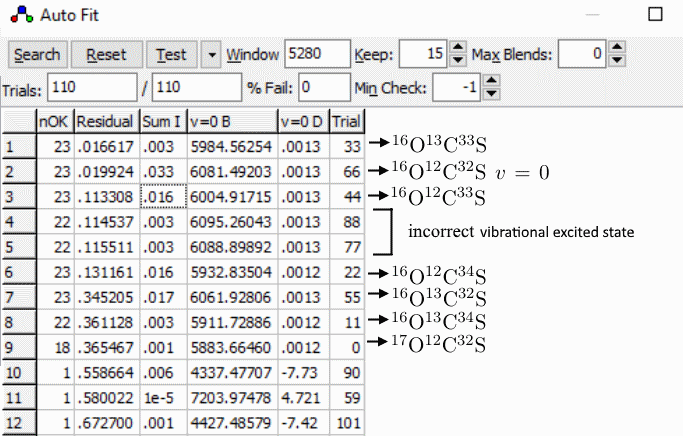
\includegraphics[width=0.85\linewidth]{./pic/ocs_first_try}}
\caption{\small Result of an OCS auto fit.}
\label{fig:ocs_first_try}
\end{figure}

If we decrease $\Delta c$ from its initial guess of $1$ MHz, $n_{OK}$ goes down for all output assignments, until we can't separate correct ones anymore. Also the differences and ratios of $n_{OK}$ between different output rows vary as $\Delta c$ changes. If we increase $\Delta c$ from  its initial guess of $1$ MHz to $3$ MHz, all isotopologues now get all 25 transitions assigned. If we increase it further, the incorrectly treated vibrationally exited transitions also get all transitions assigned (since they obey the same model except for L-doubling, they cannot be separated here). Starting with a value of about $500$ MHz, we cannot separate correct assignments from wrong ones by $n_{OK}$.

We expected that increasing the number of check transitions ($|C|$) and,  simultaneously, increasing $\Delta c$ makes the correct assignments even more separable from the incorrect. And indeed, with $|C| = 40$ and $\Delta c = 10$ MHz, we get almost the same situation as for $|C| = 25$, $\Delta c = 2$ MHz, except that the $n_{OK}$ difference between the right and the wrong has grown to $33$.

We also tried increasing $|C|$ and, simultaneously, adding $H$ to the fit (without changing $\Delta c$). But $H$ is poorly defined from least squares even for $|C| = 40$, and AUTOFIT gives \lq\lq{}rubbish out\rq\rq{}: check transitions are assigned poorly and he Residuals window shows seemingly even larger errors than with only $B$ and $D$ being fitted.

In the third test, we generated spectrum of $\rm ^{16}O^{12}C^{32}S$ $v = 0$ with added random normal errors with $\sigma = 0.1$ MHz to CDMS line positions. %Intuition may suggest that with a $\Delta c = 1$ MHz check transitions would be assigned with $4 \sigma$ confidence or $21--22$ from $23$ check lines. That would be the case if the assignment of search transitions yielded a perfect $M$, so that each check transition would be in the exact theoretical position ($x_0$). 
Since only the 2 fit transitions are fitted in an auto fit, the model gets drastically worse with errors introduced into search transitions. In our case, the higher frequency check transitions get large systematic deviations, but, again, increasing $\Delta c$ allowed to assign all check transitions correctly. The strategy of increasing $\Delta c$ worked also in the next test, where $1000$ random \lq\lq{}weeds\rq\rq{} were added to the spectrum (Fig. \ref{fig:weeds}).

\begin{figure}[h]
\center{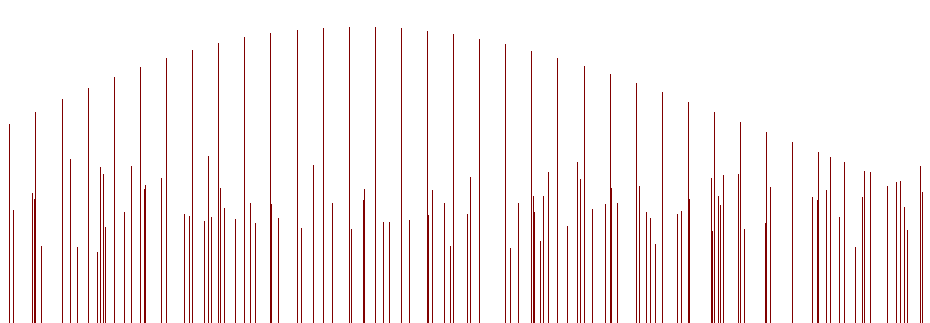
\includegraphics[width=0.85\linewidth]{./pic/weeds}}
\caption{\small A piece of OCS spectrum showing main species in ground vibrational state with additional random \lq\lq{}weed\rq\rq{} lines and random normal noise in line positions.}
\label{fig:weeds}
\end{figure}

The last test combines all the above difficulties -- several species of $\rm OCS$ put together, mixed with \lq\lq{}weeds\rq\rq{} and with added random normal shifts of line positions. With reasonable random shift values ($\sigma = 0.1 MHz$) the correct assignments are still distinguishable in an auto fit with same fit and check transitions as in previous tests (total $40$ transitions), with $B$ and $D$ floated, $\Delta s = 5280$ MHz and upon increasing the check window up to $\Delta c = 60$ MHz. 

As in previous tests, increasing both $\Delta c$ and $|C|$ ultimately yields $n_{OK} = 38$ for correct assignments with a  \lq\lq{}gap\rq\rq{} in $n_{OK}$ between the correct and incorrect assignments in AUTOFIT output. An additional hint particularly for this this case is to look at the similarity of $D$ in output assignments because typically higher order terms vary less then lower order terms between species of a molecule.

But there is also at least one more strategy that can be used: adding another fit transition \emph{without} adding an additional fit parameter. This reduces obs minus calc after the auto fit compared to an auto fit with fewer fit transitions and enlarges the $n_{OK}$ \lq\lq{}gap\rq\rq{}. The main disadvantage -- computation time goes up drastically. %The final output for $3$ fit transitions and $37$ check transitions with a $\Delta c = 35$ MHz is shown in Fig. \ref{fig:ocs_final}.

With all transitions up to 300 GHz assigned, we consider the early stage of assignment complete for this case. Transitions with higher frequencies can be assigned by using the Nearest method -- one only has to worry about floating additional distortions at some point. 

\subsubsection{Example - vinyl cyanide}

Vinyl cyanide ($\rm C_2H_3CN$), also known as acrylonitrile or propenenitrile, is an important molecule in space: it has been detected in the Sagittarius B2 star forming region, in dark clouds, circumstellar envelopes, in Titan atmosphere. The molecule is a highly prolate asymmetric top with $\kappa = -0.9798$ for the main isotopic species in its ground vibrational state and two nonzero electric dipole moments $\mu_a = 3.816(3)$ D and $\mu_b = 0.687(8)$ D.  

For a single species and vibrational state of $\rm C_2H_3CN$, 
%For molecules near $\kappa = -1$ the largest rigid rotor constant (typically A) is much larger than the other ones and the spectrum looks almost like a spectrum of a symmetric top.  % TODO: move to introduction
distinct $K$-ladders of $\mu_a$-type lines at different $J$ are the strong features. %The $\mu_a$-type spectra can be actually assigned straightforward, though some different assignments in the middle of a $K-$ladder may need to be tested at early stage.
It is important to float $B$, $C$ and $DJK$ in the initial auto fit, as those constants are the main factors for the mentioned $K$-ladders. 


For the same reason as in the OCS example, we took here artificial mixtures of $\rm C_2H_3CN$ lines from CDMS. In the first test, just the main species was taken as $E$ and one asymmetric top model was created in PGOPHER with only rigid rotational constants $A, B, C$. The initial constant values were derived from true values of a complete parameter list by forcefully setting all distortions and perturbations to zero and then fitting the correct assignment to only $A, B, C$. This gives, in some sense, effective values of $A, B, C$, which mimic ab initio calculation results. %selecting random shifts within $1\%$ of the true value, resembling an ab initio calculations result, where also $1\%$ error is often a fair guess. 

At the early stage of assignment is it reasonable to start again below and around $100$ GHz. We were going to try the brute force approach again and put $\mu_a$-type transitions with $6 \leq J' \leq 14$, with $10\%$ strength cutoff and 140 GHz frequency cutoff (total of 165 transitions), preliminary marked as check transitions, into the Line List.  

%The fit transitions set must have enough  \lq\lq{}diversity\rq\rq{}\todo{what the heck is diversity}  in quantum numbers to minimize the uncertainty after a least squares fit. In respect to that good fit transitions with a fixed total amount may be suggested automatically -- the original AUTOFIT software has this feature. A right thumb approach to this would be to select fit transitions from different K-ladders (i.e. with different $J'$).

Different sets of fit transitions in this test, unlike the simple case of $\rm OCS$, yield considerably different output, although some predicted lines are assigned to the same experimental peaks among several auto fits with different fit transitions. It seems like for this case and more complex cases, visual instruments and human judgment are needed to distinguish \lq\lq{}almost correct\rq\rq{} assignments.

In our case with $\rm 9_{2,7}-8_{2,6}, 9_{1,8}-8_{1,7}, 10_{1,10}-9_{1,9}$ as fit transitions, $2000$ MHz search window and $20$ MHz check window we get a following good and well distinguishable assignment in the first output row. 

The next stage of assignment, the intermediate stage, begins then. Typically it is reasonable to use the Nearest Lines instrument for visualizing the trend of the R-branch lines first, when working in PGOPHER. The Nearest Lines instrument in our case shows a mess when selecting all Kas together, but you can see some trends when selecting individual Kas. There, when viewing a +-1 MHz by 190 GHz window, Ka=1,2,3 have a large curvature, Ka=3,4,5,6 look ok, and Ka >= 8 trends become a large Y axis shift, and that shift is rapidly increasing with increasing Ka, so that for large Kas the correct assignement points are completely out of visibility. 

What also can be noticed is that for some lower Kas the lines are in a sense isolated, so that in a reasonable search window only one experimental peak corresponds to a given transition immediately after AUTOFIT or even before (with only ab initios). These transitons can be assigned right away. But it is not done automatically by now, since the automatic routines are not sure when there is really only one possible candidate, and this decision is left to the human, the humans eye is very good at recognizing patterns. 

Patterns consist of calc transitions repeatedly positioned together at different quantum numbers. There are true patterns and false patterns. Also, already assigned lines from the current species or other isotopologues and vibrational states play a big role. And also the intensity ratios play a big role, thought only locally, and only ratios, not the absolute intensities, for most experiments done, algthough there are experiments which are calibrated to absolute intensities.
 
\subsubsection{Example - thiazole}

Thiazole is a ring molecule, well known in infrared, whose vibrationally excited rotation states had not been investigated before. In this work, new analysis methods are applied to their investigation.

At first we do an AUTOFIT run. We want to fit only $B$ and $C$ to the a-type spectrum, but selecting only two fit transitions doesn't give a good result. \todo{Provide a proof for this using vinyl cyanide.} Then we use $3$ fit transitions. 

After selecting the correct result from AUTOFIT output, the middle stage of assignement begins. For the ground vibrational state of the main isotopologue, which has the strongest lines, the middle stage of assignment was quite simple, because in the Nearest Line Plot the trend was immediately visible. That was, however, not the case with v18=1 and even less with v17=1. For these states, some manual search for good assignments and their neighbourhoods were needed.

So it is obvious that an automated procedure should respect already assigned lines from the main species (and others.)
%\begin{figure}[h]
%\center{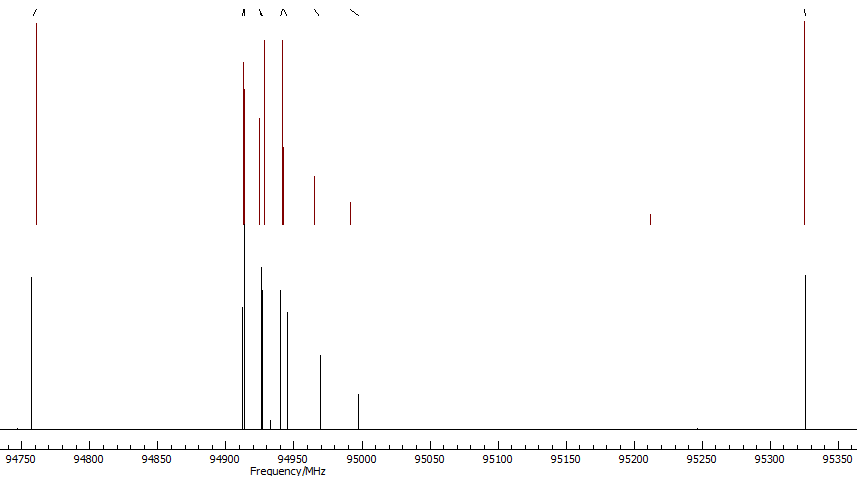
\includegraphics[width=0.85\linewidth]{./pic/vyn_first}}
%\caption{\small The fist step of the early stage assignment of  $\rm C_2H_3CN$ main species (1st test). }
%\label{fig:vyn_first}
%\end{figure}

%The next step would be to add more lines and more fit parameters to the model, possibly re-assigning incorrect assigned lines. Using the Nearest button, we add further $\mu_a$-type lines up to $J' = 19$ with the same Acceptance of $20$ MHz. The residuals in Residuals window are rather uniformly spread with an average of $7.8$ MHz over 300 line positions (most of them are 2-fold degenerate). 


%In the second test, the following mixture was prepared:
% \begin{itemize}
%	\item the main species in ground vibrational state at 100\% CDMS line strength
%	\item 4 isotopologues with a single substituted $\rm ^{13}C$ at 25\% CDMS line strength
%\end{itemize}


%Colin Western in the manual recommends to select $\Delta c$ according to the instrumental resolution. For pure rotational transitions, a better start might be $\Delta s / 10$. It is also good to select $\Delta B$ proportional to $\Delta s$ and inversely proportional to $J$ (because of the formula). Setting $\Delta B$ nonzero saves a lot of calculation time in PGOPHER, about 10 times faster in our case.  

%Observation: when decreasing check window size keeping everything else as it is, fist of all, nOK decreases, but the correct answer is still at the top. But then some wrong assignments can get to the top 20 rows. This supports the idea that when $\Delta c$ is less then the deviation arising from still closed constants, "correct" lines are not assigned, and the right answer competes with wrong ones.

%[Also observation 4, hypothesis 5 and 6. and 7]

\subsubsection{Example - 3-methylbutyronitrile}


\subsection{Nearest Lines Plot}


\subsection{SCANNER}


%\subsubsection{Example - Methylbutyronitrile}

\section{The way towards automated experiments}

\subsection{SURFER}

\section{Conclusion}

%\subsection{Vinyl cyanide reference}

%\subsection{Methylbutyronitrile reference}

%\subsection{Software user manuals}


\end{document}
